\chapter{Simulation}
\label{annex:detectors-sc-physics-software-simulation}

Simulated data samples provide the basis for detailed studies of detector performance, inform
detector design choices,  and enable the development of automated event reconstruction.
Detailed Monte Carlo predictions of expected data distributions will also be needed
in order to extract physics results from the DUNE experiment.   Several important sources
of systematic uncertainty come from detector modeling, and varying the assumptions incorporated
in the simulations provides the mechanism by which these systematic uncertainties can be estimated.
Simulations are needed in order
to extrapolate from auxiliary data samples, such testbeam measurements or {\it in situ} measurements
using events not passing signal event selection requirements, to the signal selection samples.
The following sections describe the simulation of the Near and Far Detectors.

\section{Near Detector Simulation}
\label{annex:detectors-sc-physics-software-simulation-nd}

\fixme{To be supplied, even if short}

\section{Far Detector Simulation}
\label{annex:detectors-sc-physics-software-simulation-fd}

\begin{cdrfigure}[Far detector simulation block diagram]{fdsimblockdiag}
{Block diagram showing the components of the far detector simulation chain}
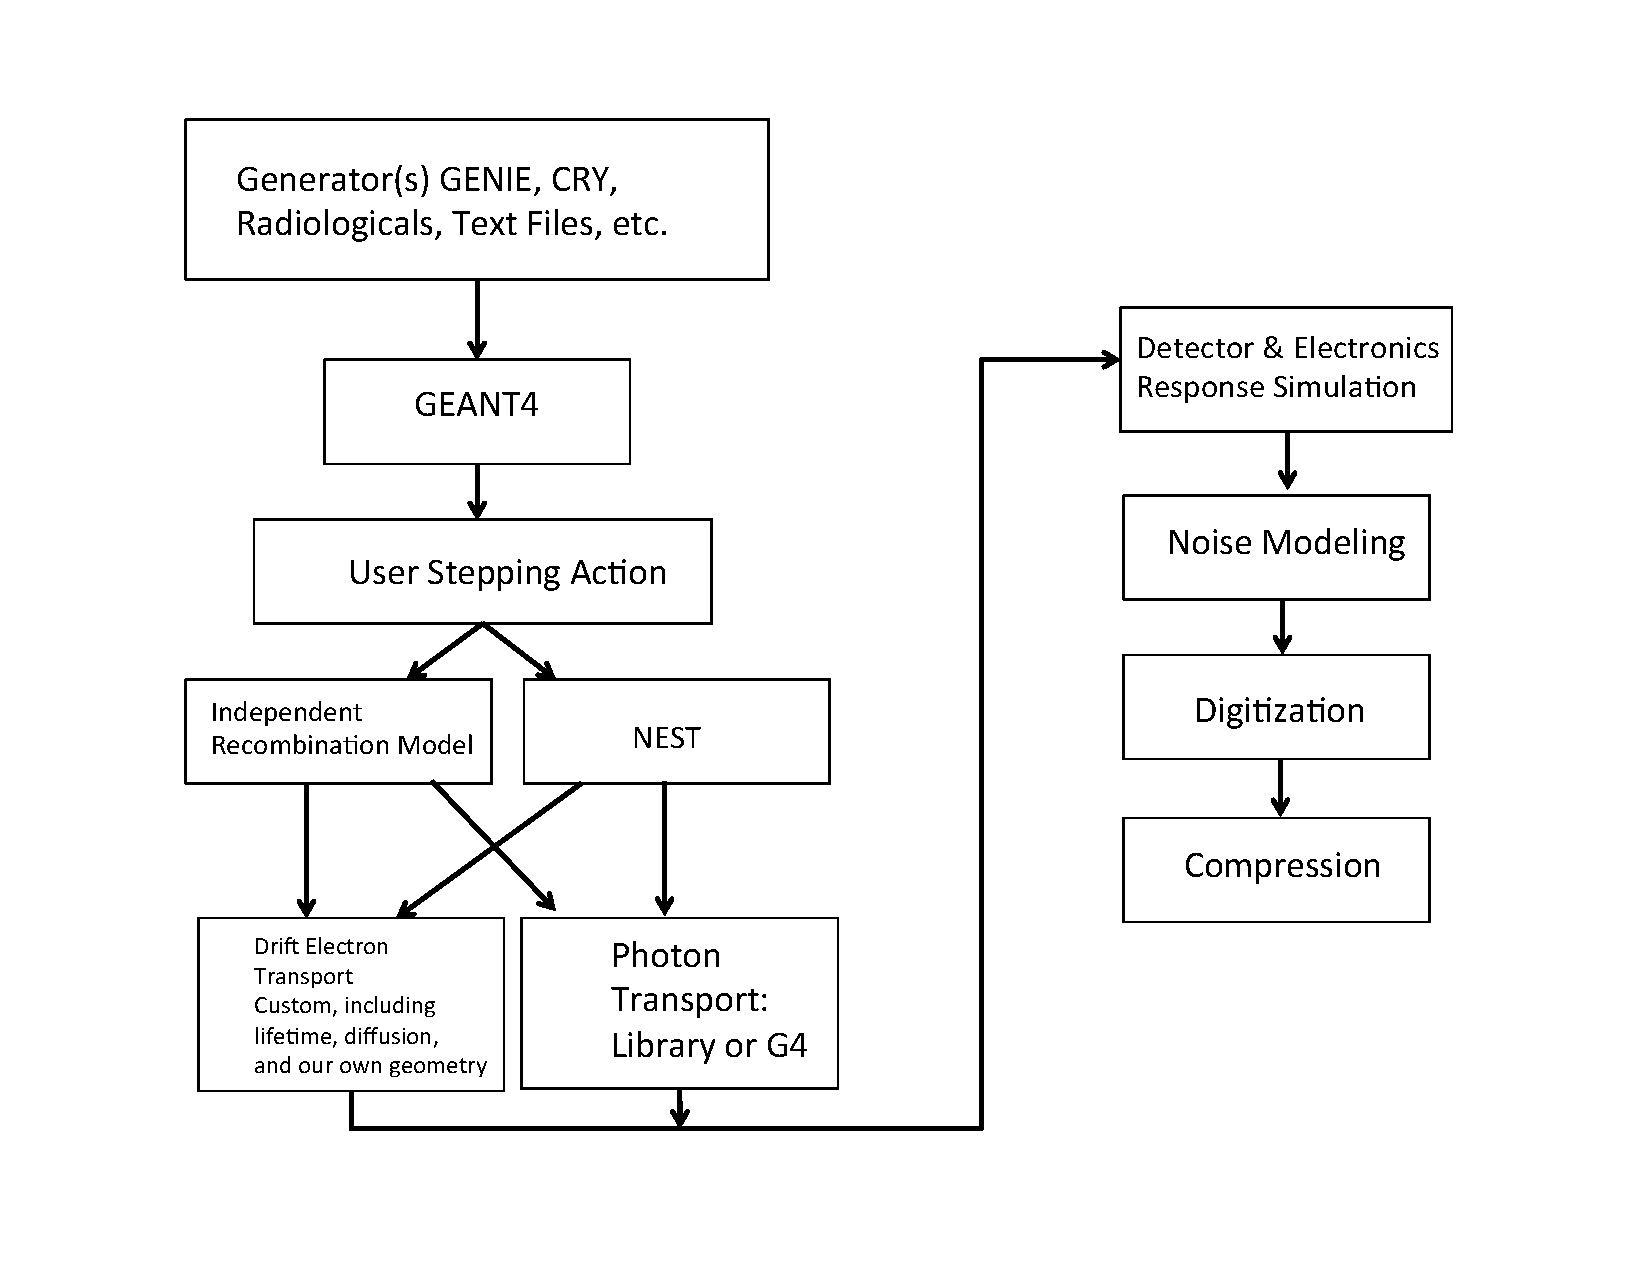
\includegraphics[width=0.95\textwidth]{fdsimflowchart_annex.pdf}
\end{cdrfigure}

Monte-Carlo simulations of liquid-argon TPC detectors have reached a level of maturity
in the last decade.  Detailed GEANT4-based~\cite{GEANT4:NIM,GEANT4} simulation
programs have been developed  for both the single-phase and dual-phase Far Detector designs,
incorporating both the Liquid Argon TPC modules and the photon detection systems.   

The single-phase detector simulation is implemented in LArSoft,
which provides a common simulation framework for Liquid Argon TPC experiments.
Confidence in the simulation capabilities is improved by
the comparison of data from ArgoNeuT~\cite{Adamson:2013/02/28tla,argoneut-url,Acciarri:2013met,Anderson:2012mra} with LArSoft
simulations.  Future data from LArIAT~\cite{Adamson:2013/02/28tla,Cavanna:2014iqa},
MicroBooNE~\cite{Chen:2007ae,Jones:2011ci,microboonecdr}, and the 35-ton prototype will allow
further tuning of the LArSoft simulation as experience is gained.
The dual-phase detector simulation is based on the Qscan package,
which has been developed over the past decade, and is currently
being used to perform technical design and physics studies for
the WA105 program.

Events are generated using the GENIE~\cite{GENIE} neutrino-nucleus
simulation program, the CRY~\cite{Cosmic-CRY,Cosmic-CRY-protons,CRY-url} 
cosmic-ray generator, a custom radiological decay simulator, a particle gun, or one of several
text-file-based particle input sources.  The interactions of particles
with the liquid argon and other detector materials is simulated with
GEANT4.  A flexible geometry description interface is provided using
GDML~\cite{gdml} files that can be altered as the detector design
evolves.  GEANT4 is used to simulate energy deposits in each step of
each particle, and custom routines have been written to translate
these into numbers of ionization electrons and scintillation photons
produced in the liquid argon.  Two ionization models are available: a
simple parameterization that scales electrons and photons with energy
using a modified Birks recombination model~\cite{Birks:1964zz,Doke:1988dp}, and
NEST~\cite{Szydagis:2013sih,Szydagis:2011tk}, a more detailed simulation that incorporates the
expected statistical anticorrelation between scintillation photons and
drifting electrons, and which has been tuned to match available noble
liquid detector data.

\subsection{Single-Phase Detector Modeling}

The drifting electrons are propagated using dedicated code that
numerically integrates over the diffusion probabilities, includes the
effect of finite electron lifetime, and selects the wire on which to
deposit the charge.  A parameterization of the distortions expected
from average values of space charge accumulations is also modeled,
though the main impact of this will be seen in the 35-ton prototype
and liquid argon TPC detectors on the surface, such as
MicroBooNE and LArIAT.  Information is
saved in memory and written to the simulation output file of where
each parcel of charge on each wire originated, and what the GEANT
particle ID was that generated that charge.

Propagating photons are simulated using a lookup table that is filled
with the probabilities for detecting a photon in a specific detector channel
when it is emitted at a point in space, where the detector channels
and a binning of the point in space serve as indices to the lookup table.
This table is filled using fully simulated photons propagated with GEANT4, including the effects
of Rayleigh scattering, reflection, and absorption on the detector
surfaces.  
Broadening of  photons arrival time (due to multiple Rayleigh scatterings)
is also parametrised and such information can be retrieved at simulation time
to properly reproduce the features of time signal.
The detection probabilities for photons striking the
sensitive materials of the photon detectors is separately
parameterized.

Signals on the TPC wires and photon detectors are then convoluted with
the expected response functions, which include the induced charge
vs. time functions and the electronics response functions,
parameterized noise is added, and the result is saved as simulated ADC
values vs. time, where digitization is simulated at 2~MHz for the TPC
wires and 150~MHz for the photon detectors, including the effects of
saturation of the ADC's.  The bipolar induction-plane signals and the
unipolar collection-plane signals are simulated separately.  Induced
charge on neighboring collection wires has a bipolar component to it
and is added to the unipolar direct collection signal.  Events are
defined to be at least one drift window long, though much longer
events are needed in order to sample interactions that happen near the
edges in either space or time.  Zero suppression and Huffman coding of
the data are applied as options.  The data are stored in ROOT files
using the compression algorithms available in ROOT.

\subsection{Dual-Phase Detector Modeling}

In a dual-phase liquid argon detector, the TPC signal amplification 
is based on the charge multiplication in argon vapor due to the Townsend effect, 
i.e. drifting electrons gain enough energy in a strong electric field to further ionize argon atoms. 
The readout system consists of an extraction grid, a Large Electron Multiplier (LEM) and two views anode.
For such technology, additional processes contribute to the
accumulation of space charge, hence to the actual electric field in the liquid active volume.
In particular, in the charge multiplication process, there is a formation of positive argon ions, 
that drift back towards the active volume. 
A significant part is collected on the bottom electrode of the LEM and on the extraction grid. 
The ions that enter into the liquid phase contribute to the positive charge distribution.
The local value of the electric charge density and the three components of the electric field
are computed using a three-dimensional time-dependent finite element analysis calculation of the equilibrium 
configuration of a physical system where the differential equations describing each charge production (e.g.: ionisation, amplification) and
absorption (e.g.: recombination, attachment) process are solved simultaneously. 
A lookup table is then used in Qscan at simulation/reconstruction level in order to associate to a given point in the active
detector volume the channels where the charge will be deposited on the readout plane as well as the drift time.

Light readout system in the dual-phase liquid argon TPC consists of an array of cryogenic photomultipliers (PMT).
The PMT components, both the reflecting surfaces and the sesitive elements., are simulated in GEANT4.
Moreover, the PMT detector surface is coated with a layer of wavelength shifting (WLS) material which converts a
scintillation photon (optical UV photon) into a visible photon. The WLS behaviour if fully simulated in
terms of absorption probability as well as emission spectrum.
The dependence of the collection efficiency on the photon incident angle is also taken into account on the base
of the existing measurements.  

A lookup table is used to calculate the probability for a photon emitted in a
given volume element to be detected by a specific PMT.
Broadening of photons arrival time (due to multiple Rayleigh scatterings)
is also parametrised and such information can be retrieved at simulation time
to properly reproduce the features of time signal.

For each detected photon a voltage signal is simulated following the results of dedicated 
measurements showing that a typical PMT response can be approximated with a log-normal distribution.
Similarly, the charge integral of the produced signal is sampled from a distibution extracted form data obtained during calibration measurements
performed on the specific PMT model.

For the complete treatment of the light production in a dual-phase TPC
the secondary scintillation light must be taken into account as well.
Secondary scintillation process refers to light produced in the gas phase of the detector when electrons, extracted form the liquid, are accelerated.
Scintillation in argon gas is simulated through a parameterization to the existing measurements of secondary scintillation light yields.

Signal on the charge readout plane is simulated in Qscan through a waveform generation stage where the MC truth information
is converted into a readout signal. 
The finally recorded signal  is a convolution of the induced current and the response of the preamplifier.
In the case of a LEM readout, 
a collection plane that records unipolar signals,  due to the fast electron drift in gas and the short induction gap between LEM and 2D anode, 
the induced current approaches a $\delta$-function and the signal is directly given by the fast response of the preamplifier.
The recorded voltage signal is then simulated by using a preamplifier response function
as measured on small scale double phase liquid argon TPC setups. 
Noise of a given amplitude can be added on top of the signal waveforms.
Besides the generation of white noise, it is also possible to use a specific frequency spectrum that has e.g. been extracted from real data. 
The final step is the digitization of the generated waveforms.


